%% img/oracles/PPP.tex
%% Copyright 2019 Andrea Berlingieri
%
% This work may be distributed and/or modified under the
% conditions of the LaTeX Project Public License, either version 1.3
% of this license or (at your option) any later version.
% The latest version of this license is in
%   http://www.latex-project.org/lppl.txt
% and version 1.3 or later is part of all distributions of LaTeX
% version 2005/12/01 or later.
%
% This work has the LPPL maintenance status `maintained'.
%
% The Current Maintainer of this work is Andrea Berlingieri.
%
% This work consists of all files listed in manifest.txt
\documentclass{standalone}

\usepackage{../TikzStyle}
\usepackage{../mystyle}
%\usetikzlibrary{decorating}
\usetikzlibrary{positioning}

\begin{document}
    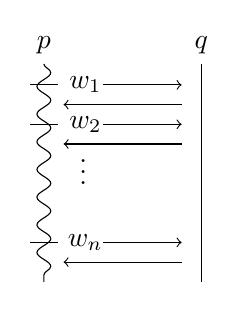
\begin{tikzpicture}
        \node (p) at (0,0) {$p$};
        \node (q) at (2,0) {$q$};
        \draw[decorate,decoration=snake] (p) -- (0,-3);
        \draw (q) -- (2,-3);
        \draw (-5pt,-0.5) -- (5pt,-0.5) node [pos=2] {$w_{1}$};
        \draw[->] (0.75,-0.5) -- (1.75,-0.5);
        \draw[->] (1.75,-0.75) -- (0.25,-0.75);
        \draw (-5pt,-1) -- (5pt,-1) node [pos=2] {$w_{2}$};
        \draw[->] (0.75,-1) -- (1.75,-1);
        \draw[->] (1.75,-1.25) -- (0.25,-1.25);
        \node () at (0.5,-1.5) {$\vdots$};
        \draw (-5pt,-2.5) -- (5pt,-2.5) node [pos=2] {$w_{n}$};
        \draw[->] (0.75,-2.5) -- (1.75,-2.5);
        \draw[->] (1.75,-2.75) -- (0.25,-2.75);
    \end{tikzpicture}
\end{document}
